\section{Bounding Circles}
A circle is the simplest form of an intersection bounding shape. This
simplicity arises from the fact that a circle is defined solely by its center
and radius, which makes calculations for collision detection more
straightforward.
\begin{figure}[H]
    \begin{center}
        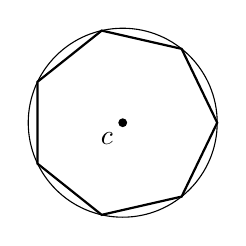
\begin{tikzpicture}

            \begin{scope}[yscale=-1, yshift=-5cm, xshift=5cm, scale=0.4]
                \drawaxesgrid{12}{12}
                % Draw a circle with a dot in the centre
                \draw [thin] (6,6) circle (3);

                % Calculate the vertices of a heptagon (7-sided polygon)
                \foreach \i in {0,1,...,6} {
                        \pgfmathsetmacro{\angle}{360/7*\i}
                        \pgfmathsetmacro{\x}{6 + 3*cos(\angle)}
                        \pgfmathsetmacro{\y}{6 + 3*sin(\angle)}
                        \coordinate (P\i) at (\x,\y);
                    }

                % Draw the heptagon
                \draw[thick] (P0) -- (P1) -- (P2) -- (P3) -- (P4) -- (P5) -- (P6) -- cycle;

                \fill (6,6) circle (4pt) node[anchor=north east] {$c$};
            \end{scope}
        \end{tikzpicture}
    \end{center}
    \caption{A heptagon (7-sided polygon) approximated by a bounding circle}
\end{figure}

Consider a complex polygon with numerous vertices. Calculating collisions for
such a polygon can be computationally intensive. However, by approximating the
polygon with a circle, the collision detection process can be simplified
significantly.

\subsection{Point in Circle Intersection}
To determine if a point lies within a circle, we can calculate the distance
from the point to the center of the circle and compare it to the circle's
radius.

Given a circle with center $c$ and radius $r$, and a point $p$, the distance
between the point and the center is given by:

\begin{equation}
    \begin{aligned}
        d_x & = p.x - c.x                \\
        d_y & = p.y - c.y                \\
        d   & = \sqrt{{d_x}^2 + {d_y}^2}
    \end{aligned}
\end{equation}

If the distance $d$ is less than the radius $r$, the point lies within the
circle.

\begin{center}
    \textit{Point lies within circle if and only if:}\\
    $d < r$
\end{center}

\subsubsection{Example}
\begin{figure}[H]
    \begin{center}
        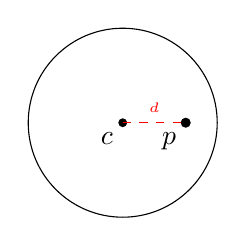
\begin{tikzpicture}
            \begin{scope}[yscale=-1, yshift=-5cm, xshift=5cm, scale=0.4]
                \drawaxesgrid{12}{12}
                % Draw a circle with a dot in the centre
                \draw [thin] (6,6) circle (3);
                \fill (6,6) circle (4pt) node[anchor=north east] {$c$};

                % Draw a point
                \filldraw [black] (8, 6) circle (4pt) node[anchor=north east] {$p$};

                % Draw a line from the center to the point
                \draw [red, dashed] (6, 6) -- (8, 6);

                % Label the distance
                \node [red, anchor=south] at (7, 6) {\tiny $d$};
            \end{scope}
        \end{tikzpicture}
    \end{center}
    \caption{Point in Circle Intersection Example}

\end{figure}

Given a circle with center $c = (6, 6)$ and radius $r = 3$, and a point $p =
    (8, 6)$, use math to determine if the point lies within the circle.

\subsubsection{Mathematical Solution}

First calculate the distance between the point and the center:
\begin{equation*}
    \begin{aligned}
        \Delta_x & = 8 - 6 = 2,            \\
        \Delta_y & = 6 - 6 = 0,            \\
        \Delta   & = \sqrt{2^2 + 0^2} = 2, \\
    \end{aligned}
\end{equation*}

Now, compare the distance to the radius:
\begin{equation*}
    \begin{aligned}
        \Delta < r                 & \rightarrow \textnormal{Point lies within circle.} \\
        2 < 3                      & \rightarrow \textnormal{Point lies within circle.} \\
        \textnormal{\textbf{TRUE}} & \rightarrow \textnormal{Point lies within circle.} \\
    \end{aligned}
\end{equation*}

Since the distance between the point and the center is less than the radius,
the point lies within the circle.

\subsubsection{Code Solution}

Here is an implementation of the algorithm in C++: \vspace{1em}
\begin{mdframed}[linecolor=black!30!white,linewidth=.5pt,extratopheight=3em]
    \begin{lstlisting}[language=C++, aboveskip=3mm,
        belowskip=3mm,
        showstringspaces=false,
        columns=flexible,
        basicstyle={\small\ttfamily},
        numbers=left,
        numberstyle=\tiny\color{gray},
        keywordstyle=\color{blue},
        commentstyle=\color{dkgreen},
        stringstyle=\color{mauve},
        breaklines=true,
        breakatwhitespace=true,
        tabsize=3,
        xleftmargin=1em]

#include "Vec2.h"
#include <cmath>
#include <iostream>

struct Circle {
    Vec2 center;
    float radius;
};

bool pointInCircle(const Vec2 &point, const Circle &circle) {
    const float dx = point.x - circle.center.x;
    const float dy = point.y - circle.center.y;
    const float distance = std::sqrt(dx * dx + dy * dy);
    const bool inside = distance < circle.radius;

    return inside;
}

int main() {
    Circle circle = {{6, 6}, 3};
    Vec2 point = {8, 6};

    if (pointInCircle(point, circle)) {
        std::cout << "Point lies within circle." << std::endl;
    } else {
        std::cout << "Point lies outside circle." << std::endl;
    }

    return 0;
}

\end{lstlisting}
\end{mdframed}

\subsection{Bounding Circle Intersection}

To detect if two bounding circles intersect, we must first calculate the
difference between the centers of the two circles. Given two circles with
centers $c_1$ and $c_2$ and radii $r_1$ and $r_2$, the distance between the two
centers is given by:

\begin{equation}
    \begin{aligned}
        d_x & = c_2.x - c_1.x            \\
        d_y & = c_2.y - c_1.y            \\
        d   & = \sqrt{{d_x}^2 + {d_y}^2}
    \end{aligned}
\end{equation}

This formula is derived from the Pythagorean theorem, which states that t he
length of the hypotenuse of a right triangle is given by the square root of the
sum of the squares of the two other sides.

\begin{equation}
    c = \sqrt{a^2 + b^2}
\end{equation}

Once we have the distance between the centers, we can determine if the circles
intersect by comparing this distance to the sum of their radii.

\begin{center}
    \textit{Circles intersect if and only if:}\\
    $d < r_1 + r_2$
\end{center}

\subsubsection{Example}
\begin{figure}[H]
    \begin{center}
        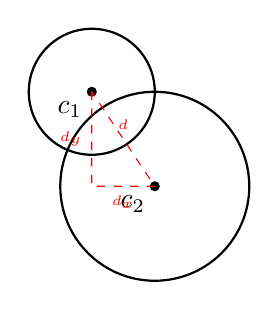
\begin{tikzpicture}
            \begin{scope}[yscale=-1, yshift=-5cm, xshift=5cm, scale=0.4]
                \drawaxesgrid{12}{12}
                % First circle
                \draw [black, thick] (5, 4) circle (2);
                % a point at the center of the first circle
                \filldraw [black] (5, 4) circle (4pt) node[anchor=north east] {$c_1$};
                % Second circle
                \draw [black, thick] (7, 7) circle (3);
                % a point at the center of the second circle
                \filldraw [black] (7, 7) circle (4pt) node[anchor=north east] {$c_2$};

                % Draw triangle representing dx, dy, d
                \draw [red, dashed] (5, 4) -- (5, 7) -- (7, 7) -- cycle;

                % Label dx, dy, d
                \node [red, anchor=east] at (5, 5.5) {\tiny $d_y$};
                \node [red, anchor=north] at (6, 7) {\tiny $d_x$};
                \node [red, anchor=south] at (6, 5.5) {\tiny $d$};

            \end{scope}
        \end{tikzpicture}

        \caption{Bounding Circle Intersection Example}
    \end{center}
\end{figure}

Given two circles with centers $c_1 = (5, 4)$ and $c_2 = (7, 7)$ and radii $r_1
    = 2$ and $r_2 = 3$, use math to determine if the circles intersect.

\subsubsubsection{Mathematical Solution}
First calculate the distance between the two centers:
\begin{equation*}
    \begin{aligned}
        \Delta_x & = 7 - 5 = 2,                                 \\
        \Delta_y & = 7 - 4 = 3,                                 \\
        \Delta   & = \sqrt{2^2 + 3^2} = \sqrt{13} \approx 3.61, \\
    \end{aligned}
\end{equation*}

Now, compare the distance to the sum of the radii:
\begin{equation*}
    \begin{aligned}
        \Delta < r_1 + r_2         & \rightarrow \textnormal{Circles intersect.} \\
        3.61 < 2 + 3               & \rightarrow \textnormal{Circles intersect.} \\
        \textnormal{\textbf{TRUE}} & \rightarrow \textnormal{Circles intersect.} \\
    \end{aligned}
\end{equation*}

Since the distance between the two centers is less than the sum of the radii,
the two circles intersect.

\newpage
\subsubsubsection{Code Solution}
Here is an implementation of the collision detection algorithm in C++:
\vspace{1em}
\begin{mdframed}[linecolor=black!30!white,linewidth=.5pt,extratopheight=3em]
    \begin{lstlisting}[language=C++, aboveskip=3mm,
        belowskip=3mm,
        showstringspaces=false,
        columns=flexible,
        basicstyle={\small\ttfamily},
        numbers=left,
        numberstyle=\tiny\color{gray},
        keywordstyle=\color{blue},
        commentstyle=\color{dkgreen},
        stringstyle=\color{mauve},
        breaklines=true,
        breakatwhitespace=true,
        tabsize=3,
        xleftmargin=1em]
#include "Vec2.h"
#include <cmath>
#include <iostream>

struct Circle {
    Vec2 center;
    float radius;
};

bool checkCollision(const Circle &c1, const Circle &c2) {
    const float dx = c2.center.x - c1.center.x;
    const float dy = c2.center.y - c1.center.y;
    const float distance = std::sqrt(dx * dx + dy * dy);
    const float sumOfRadii = c1.radius + c2.radius;
    const bool collision = distance < sumOfRadii;

    return collision;
}

int main() {
    Circle c1 = {{5, 4}, 2};
    Circle c2 = {{7, 7}, 3};

    if (checkCollision(c1, c2)) {
        std::cout << "Collision detected!" << std::endl;
    } else {
        std::cout << "No collision detected." << std::endl;
    }

    return 0;
}
\end{lstlisting}

\end{mdframed}

\newpage
